\chapter{Results and Conclusions}
\section{Results}
In order to derive expected upper limits on the signal strength of the 2HDM+a samples, the likelihood function in \cref{eq:likelihood} is calculated by taking the product of the Poisson probability of the expectation value in each bin. Nuisances are calculated in each bin from the systematic uncertainties using a log-normal distribution.
\begin{equation}
    L(\mu, \boldsymbol{\theta}) = \prod_{j=1}^N\frac{(\mu s_j+b_j)^{n_j}}{n_j!}e^{-(\mu s_j+b_j)}\prod_{k=1}^M\frac{(u_k)^{m_j}}{m_j!}e^{-(u_k)}
    \label{eq:likelihood}
\end{equation}
Here, $s_j$ and $b_j$ are the mean contributions from the signal and background in the bin $j$, which is one of the $m_\text{AK8} = 100\text{--}\GeV{150}$ bins with a number of entries $n_j$. $u_k$ is the mean contribution from the other signal regions $k$ with number of entries $m_k$, which are used to get a handle on the backgrounds in the thesis. In general, these expectation values are dependent on some combination of the nuisances, denoted $\boldsymbol{\theta}$.
The profile likelihood ratio is then calculated by taking the ratio
\begin{equation}
    \frac{L(\mu=1, \boldsymbol{\hat{\hat{\theta}}})}{L(\mu=0, \boldsymbol{\hat{\hat{\theta}}})},
    \label{eq:ratio}
\end{equation}
where $\boldsymbol{\hat{\hat{\theta}}}$ is the value of $\boldsymbol{\theta}$ that maximizes $L$ for the given $\mu$.
Using the asymptotic approximation~\cite{Cowan_2011} for the test statistic described in~\cref{eq:q}, p-values for the hypotheses $\mu=1$ and $\mu=0$ were calculated using~\cref{eq:psb,eq:pb}, respectively. Here, $\sigma_{s+b}$ and $\sigma_{b}$ are the standard deviations of $q$ for the $\mu=1$ and $\mu=0$ hypotheses, respectively, which can be calculated from a covariance of $\mu$ and $\boldsymbol{\theta}$. 
\begin{equation}
    q = -2\ln\frac{L(\mu=1, \boldsymbol{\hat{\hat{\theta}}})}{L(\mu=0, \boldsymbol{\hat{\hat{\theta}}})}
    \label{eq:q}
\end{equation}
\begin{equation}
    p_{s+b} =  1 - \Phi\bigg(\frac{q_\text{obs}+\frac{1}{\sigma^2_{s+b}}}{2/\sigma_{s+b}}\bigg)
    \label{eq:psb}
\end{equation}

\begin{equation}
    p_{b} =  1 - \Phi\bigg(\frac{q_\text{obs}-\frac{1}{\sigma^2_{b}}}{2/\sigma_{b}}\bigg)
    \label{eq:pb}
\end{equation}
The significance is calculated by transforming $1-p_{s+b}$ to the respective quantile that value falls into.
Expected upper limits were calculated using the $CL_s$ test described in~\cite{Junk_1999, Read_2002}. A value for $\mu$ is determined to be the upper limit if it is the largest value for which the ratio $CL_s$, given in \cref{eq:cls}, is equal to 0.05, giving a 95\% $CL_s$ upper limit. 

\begin{equation}
    CL_s = \frac{p_{s+b}}{1-p_{b}}
    \label{eq:cls}
\end{equation}

These results were compared to those in \cite{cms:hbb2019} by applying the baseline selections to the events with an additional requirement that the mass of the highest-momentum AK8 jet be within $\GeV{25}$ of $m_\mathrm{h}$. A likelihood function is then calculated by binning events in \ptmiss in a manner similar to the analysis of the 2016 Run 2 dataset. The expected limits were within 10\% of the previous results for the 2HDM+a signal with $m_\mathrm{A} = \GeV{1000}$, $m_\mathrm{a} = \GeV{150}$. This level of agreement is reasonable considering the changes in process cross-section due to the difference in beam energy, which is demonstrated for the given signal in \cref{tab:sxsec}. In addition, there were differences in the background yields from the differences in object reconstruction and event selection.

\begin{table}
    \small
    \centering
    \caption{Cross-sections of the 2HDM+a signal for the $m_\mathrm{A} = 1000$ GeV, $m_\mathrm{a} = 150$ GeV mass point as a function of the beam energy.}
    \begin{tabular}{|c|c|c|}
        \hline
        Signal & cross-section (pb) & CoM Energy \\
        b$\bar{\mathrm{b}}$ $\to$ A, $m_\mathrm{A} = 1500$ GeV, $m_\mathrm{a} = 150$ GeV  &   $0.0004232 \pm 0.000001942$ & 13 TeV \\
        gg $\to$ A, $m_\mathrm{A} = 1500$ GeV, $m_\mathrm{a} = 150$ GeV  &          $0.03943 \pm 0.0001792$ & 13 TeV \\
        b$\bar{\mathrm{b}}$ $\to$ A, $m_\mathrm{A} = 1500$ GeV, $m_\mathrm{a} = 150$ GeV  &   $0.0005006 \pm 0.000004345$ & 14 TeV \\
        gg $\to$ A, $m_\mathrm{A} = 1500$ GeV, $m_\mathrm{a} = 150$ GeV  &          $0.04672 \pm 0.0001779$ & 14 TeV \\
        \hline
    \end{tabular}
    \label{tab:sxsec}
\end{table}


The upper limits for 3 mass scans of $m_\mathrm{a} = 250$, $500$, and $\GeV{750}$ are shown in \cref{fig:limits}. For $m_\mathrm{a} = \GeV{250}$, mass values for $m_\mathrm{A}$ between $750$ and $\GeV{2000}$ would be excluded. For $m_\mathrm{a} = \GeV{500}$, mass values for $m_\mathrm{A}$ between $1250$ and $\GeV{1600}$ would be excluded. However, $m_\mathrm{A}$ values for $m_\mathrm{a} = \GeV{750}$ cannot yet be excluded. The improvement in the range of excluded masses is driven by the increased dataset given by the HL-LHC as well as the upgraded CMS Phase-2 detector.

\begin{figure}[ht]
\centering
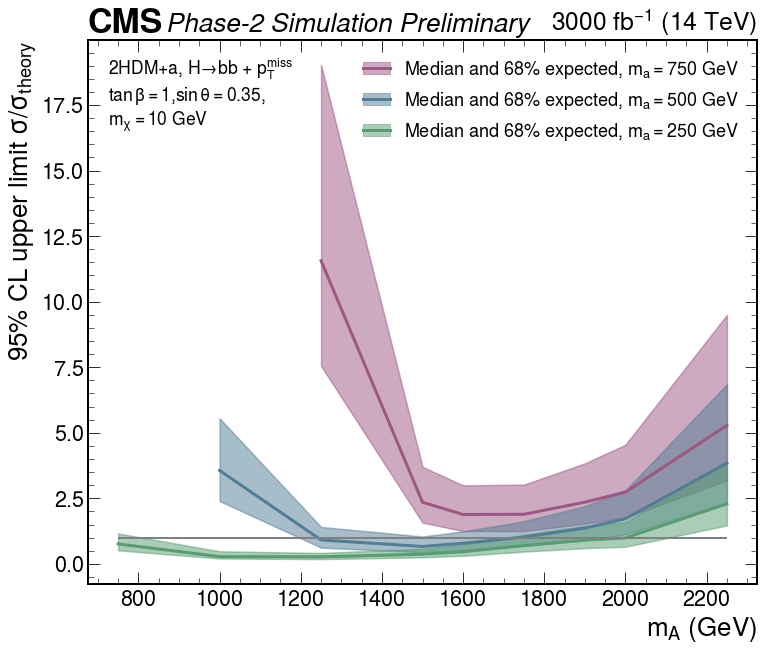
\includegraphics[width=0.5\textwidth]{Chapters/Results/lim_scan.png}
\caption{The expected limits on the 2HDM+a model of DM production in association with h $\to$ b$\bar{\mathrm{b}}$+\ptmiss. The 2HDM+a model parameters have been set at $\tan\beta = 1$, $\sin\theta = 0.35$, and $m_\chi= \GeV{10}$. The shaded regions give the 1$\sigma$ uncertainty in the limit.}
\label{fig:limits}
\end{figure}

For $m_\mathrm{a} = \GeV{250}$ and $m_\mathrm{A}$ between $1000$ and $\GeV{1600}$, the expected significance of these points could be at or above 5$\sigma$ if a significant excess is observed, as shown in \cref{fig:sig}.

\begin{figure}[ht]
\centering
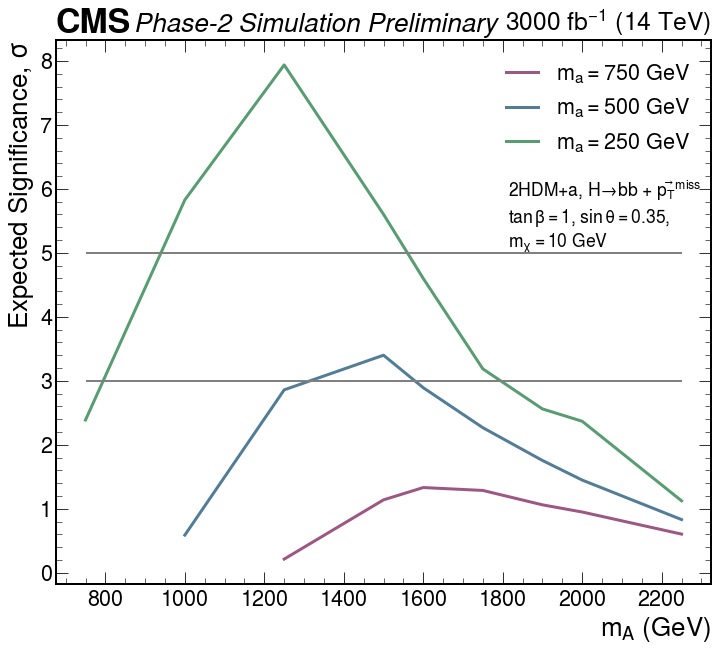
\includegraphics[width=0.5\textwidth]{Chapters/Results/sig_scan.png}
\caption{The expected significance of the 2HDM+a model of DM production in association with h $\to$ b$\bar{\mathrm{b}}$+\ptmiss. The 2HDM+a model parameters have been set at $\tan\beta = 1$, $\sin\theta = 0.35$, and $m_\chi= \GeV{10}$.}
\label{fig:sig}
\end{figure}

\section{Conclusions}
The HL-LHC will have increased sensitivity to new physics. In particular, a search probing a mono-Higgs plus \ptmiss final state where the Higgs decays to a b quark-antiquark pair will have greater sensitivity to new physics than before. Because of the increased luminosity of the collider, it is possible to probe regions that would have suffered from large statistical uncertainties, bringing further resolution to constraints on parameters of these models. The Phase-2 upgrades to CMS will allow the detector to handle the increased luminosity of the detector, ensuring the sensitivity at the HL-LHC is equal or greater than during Run 2. Additionally, upgrades to the geometry and improvements to the detector systems will allow for better exclusion of backgrounds to many searches for new physics, further increasing the sensitivity. In the case of the h $\to$ b$\bar{\mathrm{b}}$+\ptmiss final state, this analysis indicates that the expected limits would allow for further exclusion of parameter masses while establishing the first limits on higher values of the mass of the pseudoscalar A. In the case of observation of excess at the HL-LHC, there is a region of the parameter space for which this observation would be a discovery-level significance. This search could also be expanded upon. The lower mass parameter space could be explored by looking at lower-momentum Higgs bosons, increasing the sensitivity of the parameters for lower $m_\mathrm{A}$. Similarly, exploring final states with lower \ptmiss would increase the sensitivity of this search. Additionally, the parameter space could be explored further by varying the values of $\tan\beta$ or $\sin\theta$. Furthermore, this final state could be analyzed in terms of other models, such as the baryonic \Zp or \Zp-2HDM models. Regardless of the outcome, such a search would bring researchers closer to understanding the nature of dark matter. The mono-Higgs final state should be explored at the HL-LHC.